% !TeX root = ../thuthesis-example.tex

\chapter{ProSmith Analysis}
\label{chap:2}

\section{Introduction}

In this chapter, we will deep dive into ProSmith, the state-of-the-art model for Michaelis constant
prediction. We will examine the results in more details and see the limitations of the model. The later
chapters will aim to fix these issues and our results and analysis will be further discussed in 
Chapter \ref{chap:6}.

ProSmith offers the results in terms of MSE and correlation coefficient $r^2$.However, 
these general metrics fail to see in detail where the model perfoms well and does not. An
alternative to this is to use a hot/cold framework; hot meaning in the training set, and cold 
meaning not in the training set. As the models take two inputs: the protein sequence and 
the substrate string, we can evaluate our metrics for these 4 subgroups: hot proteins and hot substrates, 
hot proteins and cold substrates, cold proteins and hot substrates, and cold proteins and cold substrates. 
This will help evaluate the results,
especially for real world applications. Indeed, the general metrics fail to help us understand the 
capabilities of a model in the field of drug design.

Hot proteins and hot substrates means that proteins and the substrates are in the training set. It would
be useful to adapting existing drugs to new problems. Hot proteins and cold substrates indicates that
the proteins are in the training set but the substrates are not. This could improve the research on the
use of new chemical compounds on existing enzymes. Cold proteins and hot substrates means that the proteins
are not in the training set but that the substrates are. This may be informative to see if current drugs 
could be use on new enzymes. Finally, the most interesting and promising of all is the cold proteins
and cold substrates. Indeed, this could help identify new drugs on new enzymes, which would be completely
de novo drug and enzyme design. Furthermore, this will help interpret the generalization of our models. As
there are no existing examples in the dataset, the model has to really learn the interactions between the
protein and the substrate and cannot simply use its current knownledge to overfit the data and predict
results based on the distribution of its inputs.

We expect that the best results will be obtained for the hot proteins and hot substrates subgroup, 
as both the proteins and the substrates are within the training set. This would mean that 
the model leverages its learned patterns and interactions most effectively. 
This scenario is most conducive to the model accurately predicting outcomes based on its training.

On the other hand, the worst results are anticipated for the cold proteins and cold substrates subgroup. 
This is because neither the proteins nor the substrates have been seen by the model during training, 
presenting the most significant challenge in terms of generalization. The model must rely entirely 
on the underlying principles it has learned, without direct knowledge of these specific inputs, 
making accurate prediction considerably more difficult.

We replicated ProSmith and analyze its results with our new hot/cold framework. We obtain:

\begin{table}[ht]
  \centering
  \begin{tabular}{lcccccc}
  \hline
   & \multicolumn{3}{c}{\textbf{Hot}} & \multicolumn{3}{c}{\textbf{Cold}} \\
   & Samples & MSE & R\(^2\) & Samples & MSE & R\(^2\) \\ \hline
  \textbf{Hot seq}  & 1135 & 0.534 & 0.572 & 64 & 0.678 & 0.545 \\
  \textbf{Cold seq} & 1042 & 0.635 & 0.584 & 98 & 1.143 & 0.082 \\ \hline
  \end{tabular}
  \caption{StructKm results on the test set}
  \label{tab:prosmith_results}
\end{table}

As we observe, while the general results with MSE of 0.604 and correlation coefficient of 0.563, the
cold protein and cold substrate are very dissapointing and showcase a fault in ProSmith to predict the
interactions between completely unseen proteins and substrates in the training set.

More specifically, we see that when both the protein and substrate are hot, we have better results than
the general results, which make sense as we explained above as the model can leverage its learned patterns
and interactions most efficiently. What is more surprising however is that we obtain the highest results
for the hot substrates and cold proteins, which would mean that the substrate information is more
important than the protein. However, the model should predict the Michaelis constant, which is an
indication of the interaction between the substrate and the protein. Hence, we should have lower results
for completely unknown proteins. 

We also obtain decent results for hot proteins and cold substrates, meaning that even though we don't
have the information about the substrate in the training set, the model is capable of using its 
knowledge of proteins and substrate efficiently. However, for cold proteins and cold substrates, the model
performs extremely poorly, meaning that it is not capable of generalizing for completely unseen pairs.
This becomes very problematic as this would be one of the most important point of the model. Furthermore,
it makes us question the model ability to predict the interactions between the protein and the substrate
as we get very decent results when some data is in the training set but poor performance when it is not.

This first analysis shed lights on the capabilities of ProSmith for true generalization and question its
overall abilities to predict the interaction between the protein and the substrate and to simply overfit
on the data at hand.

Hence, in the future, we will not only look at the general metrics of our models but also at these 4
additional metrics that are much more informative.

We also obtain the following results for the new test set:

\begin{table}[ht]
  \centering
  \begin{tabular}{lcccccc}
  \hline
   & \multicolumn{3}{c}{\textbf{Hot}} & \multicolumn{3}{c}{\textbf{Cold}} \\
   & Samples & MSE & R\(^2\) & Samples & MSE & R\(^2\) \\ \hline
  \textbf{Hot seq}  & 40 & 1.439 & 0.067 & 30 & 0.827 & -0.190 \\
  \textbf{Cold seq} & 1117 & 1.175 & 0.306 & 102 & 2.202 & -0.078 \\ \hline
  \end{tabular}
  \caption{StructKm results on the new test set}
  \label{tab:summary_performance}
\end{table}

Once, again, we notice that \textcolor{add results + analysis of results}

We also wanted to 
explore its ability to model the interactions between the protein and the substrate, as the Michaelis constant
is a reflection of it. As we noticed, its performance on completely unseen proteins (cold proteins) and
completely unseen substrates (cold substrates) is very low and we wanted to know if the general results were
due to a real understanding of the protein and substrate interaction or simply an overfit on the data, which
is very common with small datasets in biology-related fields.

To do so, we conducted 2 main experiements. The first one, the single amino acid mutation effect analysis,
aims at determining the ability of the model to deal with different but very similar proteins. 
The second experiment's goal is to see where the Michaelis constant distribution lies between different 
substrates.

\subsection{Single Amino Acid Mutation Effect Analysis}

Our first experiment is the single amino acid mutation effect. This experiment aims to see how the model
performs when we slightly modify the protein sequence. For each position of the sequence, we generate another
sequence with one of the remaining 19 amino acids. For example, with a protein sequence of length 500, we
will get $500\times19=9,500$ new sequences.

Considering the large number of sequences this would create, we selected 16 sequences of the test set with
8 having a very low MSE, 8 having a very high MSE, and for each of them, 2 hot proteins and hot substrates, 
2 hot proteins and cold substrates, 2 cold proteins and hot substrates, and finally 2 cold proteins and
cold substrates. This allows us to have enough different sequences to make a decent analysis and be
able to compare how it affects the results. 

Once we selected our 16 sequences and created all their mutants, we associated them with the substrate they
were originally with in the test set, hence forming sequence-substrate pairs that can be used by the ProSmith
model and can efficiently be compared to the original sequence-substrate pair.

Below we showcase these results for 2 specific proteins: 
\begin{itemize}
    \item Sequence 1860 which comes from a protein-substrate
    pair where the sequence is not in the training set (cold protein) and the substrate is in the training set 
    (hot substrate) and where the MSE is very low, meaning the Michaelis constant was well predicted.
    \item Sequence 1866 which comes from a protein-substrate pair where the sequence is not in the training set
    (cold sequence) and the substrate is in the training set (hot substrate) and where the MSE is high,
    indicating that the Michaelis constant was not well predicted.
\end{itemize}

Figures \ref{fig:seq1860} and \ref{fig:seq1866} are graphs of the results of the impact of the mutations for
each amino acid. More specifically, once we obtained the Michaelis constant predicted by ProSmith for each 
pair of mutant-substrate, we calculated the difference between the obtained value and the predicted value for the
original protein-substrate pair, and plotted the maximum variation for each amino acid

\begin{figure}
    \centering
    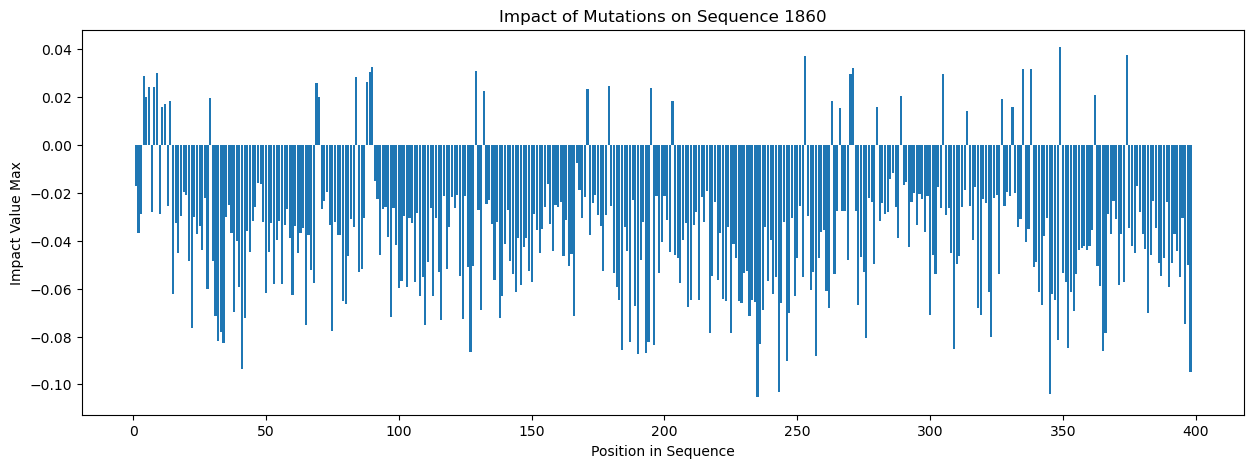
\includegraphics[width=1\linewidth]{5-small_mse_cold_hot.png}
    \caption{Single amino acid mutation effect on sequence 1860}
    \label{fig:seq1860}
  \end{figure}

\begin{figure}
    \centering
    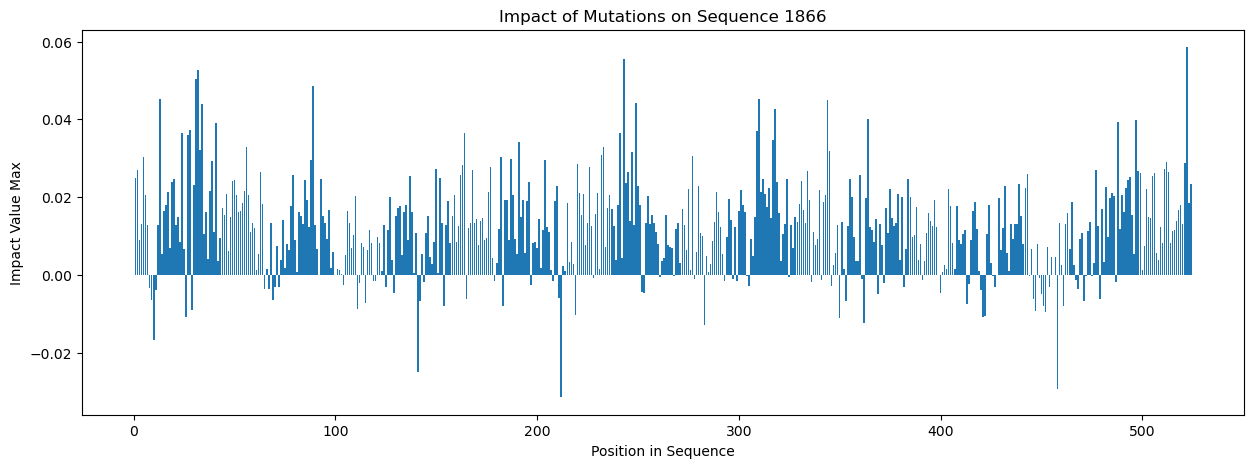
\includegraphics[width=1\linewidth]{5-high_mse_cold_hot.png}
    \caption{Single amino acid mutation effect on sequence 1041}
    \label{fig:seq1866}
  \end{figure}

We can observe 2 main elements. First, for all amino acid mutation, the variation is about the same, generally
ranging up to 0.10 (which is a maximum variation of 20\%). The second is that the variation can be positive
or negative and there is no evident pattern. These observations are essential as they provide valuable 
insights on how the model works. 

Going back to how enzymes and substrates, we know that a very small number of amino acids in the enzyme
are responsible for the reaction. This mean that one or a few amino acids are the reason why the reaction occur
and hence if the enzyme no longer has these amino acids, the reaction cannot happens and therefore, the Michaelis
constant should have an extremely high value (meaning a very low affinity). However, in our experiment, we show
that no matter what the mutation is, the value remain very close to its original prediction, meaning that the
model is not capable of capturing the interaction between the protein and the substrate.

Furthermore, as enzymes are extremely specific, we would expect that only a very small amount of sequences
show better results than the wildtype sequence: we would expect most mutant-substrate pair to have a larger
Michaelis constant (indicating a lower affinity) and only very few having a smaller Michaelis constant 
(indicating a higher affinity) that would be extremely interesting for enzyme engineering. However, as we can
see on the figures, we have positive and negative values in both directions, which does not reflect the 
reality and futher indicates the model inability to model the interaction between the enzyme and its substrate.

To continue our analysis of what the model does, we looked into the substrate distribution.

\subsection{Substrate Distribution Analysis}

Now that we looked into how the proteins impact the model prediction, which they mostly do not as the model
is not capable of predicting the interaction between the mutant and the substrate, we look into the second input:
the substrate.

In this section, we look into what we call the substrate distribution which is the Michaelis constant distribution
when focusing on the impact of the substrate. 

First of all, we wanted to know how different was the distribution of the substrates with high prediction error
compared to the general substrate distribution. In other words, we looked into how is distributed the Michaelis
constant for the substrates where the predicted Michaelis constant is far from its real value and compare it
to the global distribution of the data.

\begin{figure}
    \centering
    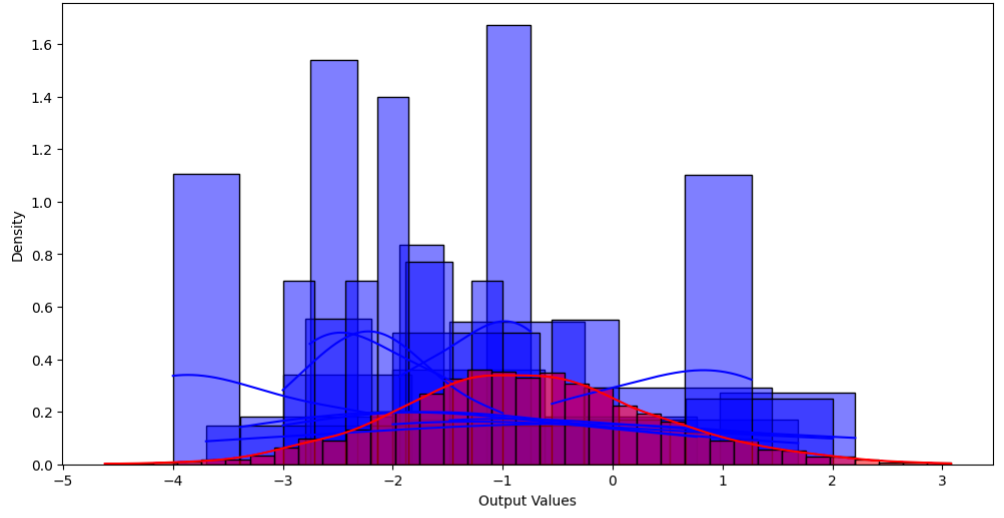
\includegraphics[width=1\linewidth]{5-substrate-dist.png}
    \caption{Distribution of the substrates with high prediction error}
    \label{fig:substratedist}
  \end{figure}

In Figure \ref{fig:substratedist}, we have in blue the substrate distribution of the 10 substrates with the
highest MSE and in red the global substrate distribution. We observe that even though these 10 substrates
have a high error, their distribution is not out of the global distribution. This means that the high error
in predicting the Michaelis constant is not due to very different substrate distribution as the high errors
do not corrolate with distribution that are outside of the global substrate distribution.

Diving deeper into the results analysis of the ProSmith model, we observe that the largest errors that are
due, either by protein-substrate pairs that are not in the training set (cold protein, cold substrate) as
indicated by the high MSE for this subset, or by substrate and proteins that are indeed in the training set
but where the Michaelis constant is far from the distribution of this specific substrate.

\begin{figure}
    \centering
    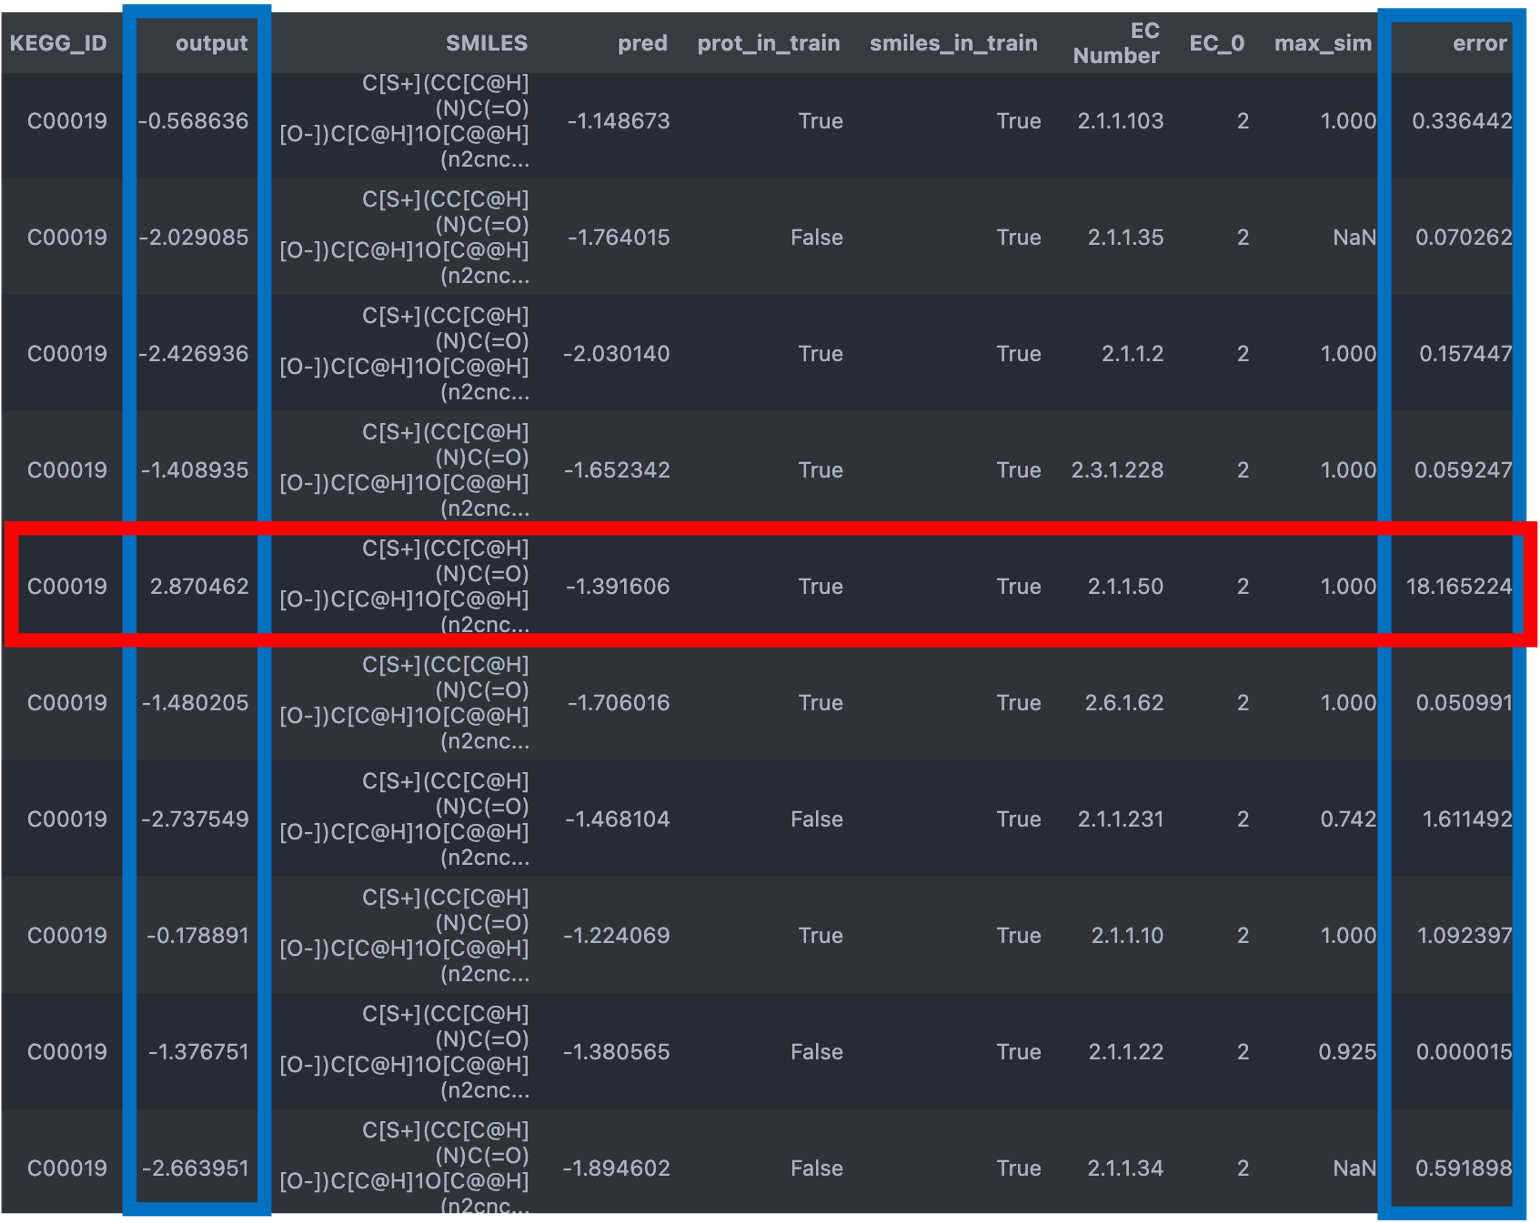
\includegraphics[width=1\linewidth]{5-results1.png}
    \caption{Results for the substrate S-Adenosylmethionine}
    \label{fig:sub1}
  \end{figure}

\begin{figure}
    \centering
    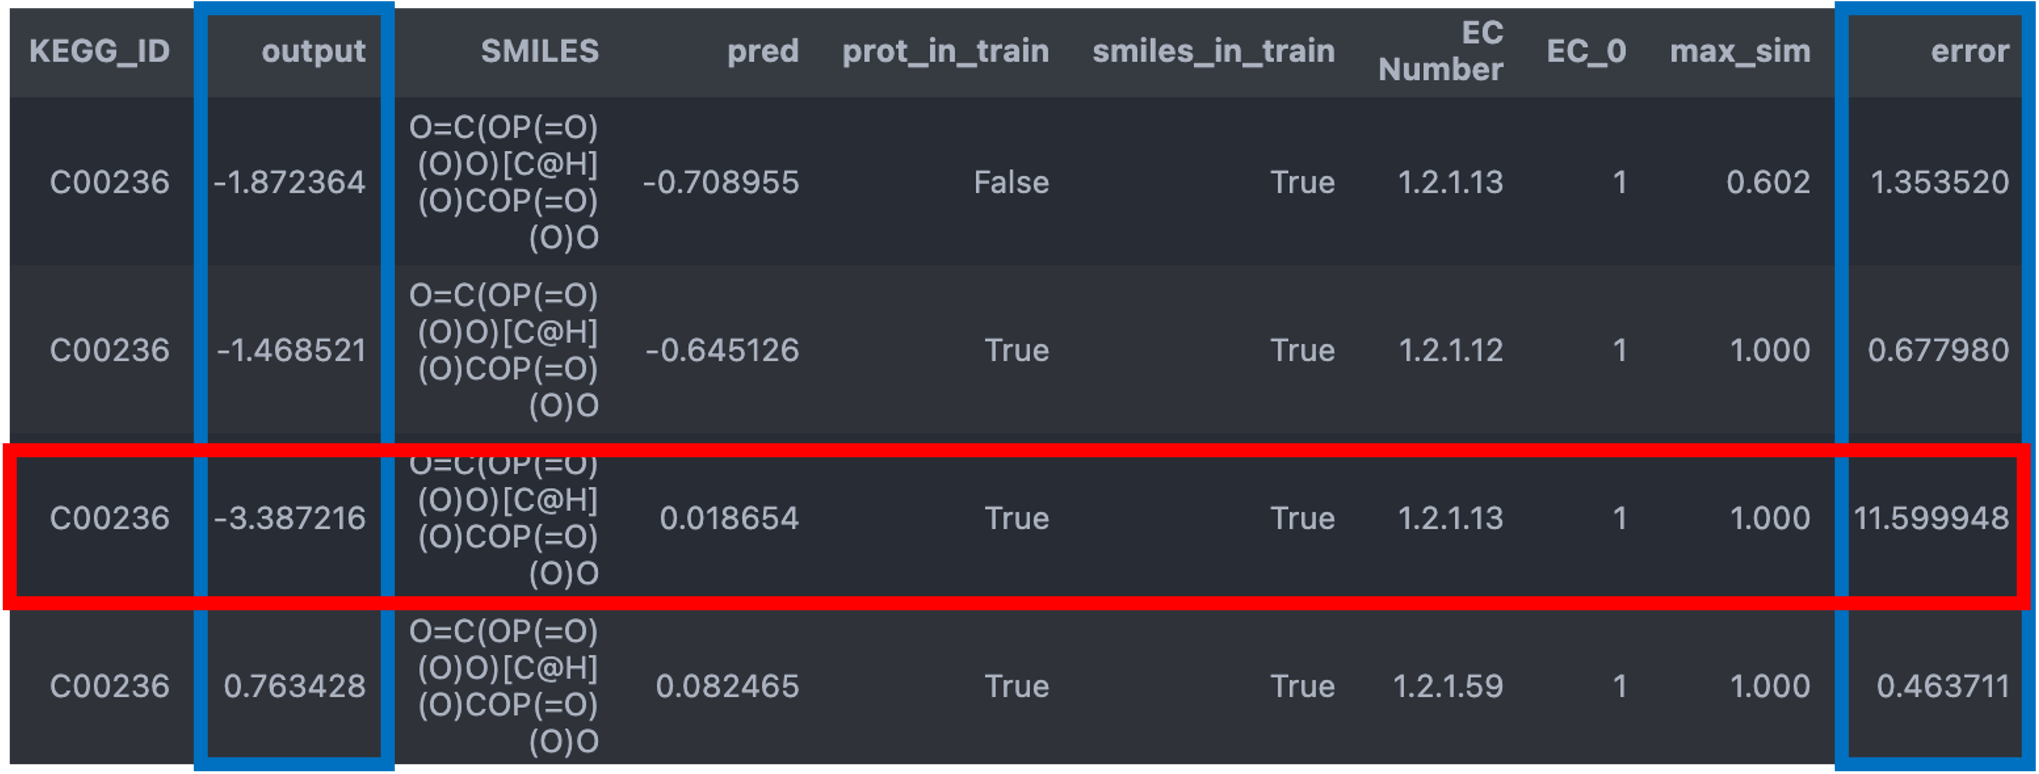
\includegraphics[width=1\linewidth]{5-results2.png}
    \caption{Results for the substrate Succinate semialdehyde}
    \label{fig:sub2}
  \end{figure}

Figures \ref{sub1} and \ref{sub2} examplify this discovery. As it is shown in red, we observe that for the same
substrate, when the real Michaelis constant is outside of the general distribution of the substrate, the model
is incapable of predicting this value properly and predicts instead a value inside the distribution of this
substrate, showing the incapability of the model to predict properly the interaction between the enzyme and
its substrate. However, this is a consequent problem as each substrate interact very differently between
different enzymes and this element is essential to take into account, which is something ProSmith is
incapable of doing.

\subsection{Analaysis Conclusions}

As we have observed, when looking in details into the single amino acid mutation analysis, we see that 
the prediction of the Michaelis constant changes within the same small range and does not take into account
the basics of biology that indicates that an enzyme which is very specific cannot offer similar performance
if we mutate all its amino acids. This indicates ProSmith's inability to model the interaction between
the enzyme and the substrate.

Furthermore, the substrate distribution analysis showcases that the highest errors are not due to substrate that
have a distribution outside of the general substrate distribution but substrate that have a normal distribution
but possess some enzymes for which the Michaelis constant is very different. This means that the model is
not capable of capturing the interactions between each protein and a substrate and bases its prediction on the
substrate distribution.

Hence, while ProSmith showcases the best performances in terms of MSE and correlation coefficient, the model
is far from being able to accurately predict the interaction between enzymes and their substrates, which indicates
clear possible improvement using different methods that will discuss in later sections. 

Moreover, these problems can be examplify by the model 0.110 correlation coefficient for cold protein and cold 
substrate, indicating that the model is not capable of generalizing properly. While our model also suffer from
this problem and offer less than optimal results with a corrolation coeffient of 0.124 for the cold proteins and
cold substrates, we outperfom ProSmith in this regard and with similar global results, we
offer a model that is capable of better generalization while maintaining decent results for the general case.
